\graphicspath{ {05-Source/Figures/} }

\section{Source}

A variety of options for the generation of the particle distribution
at source are included in the package (see
section \ref{subsubSect:A1:BLE:Source}.
The principal, and the default, option is the target-normal sheath
acceleration (TNSA) model presented in~\cite{10.1038/nphys199} .
The implementation of this model is summarised below.
The laboratory and RPLC reference frames coincide at the target,
therefore trace- and phase-coordinates are not distinguished in the
presentation of the particle-production model.

\subsection{Energy distribution}

The typical kinetic energy, $K$, spectrum produced in target-normal
sheath acceleration falls exponentially with kinetic energy before
dropping rapidly to zero above a maximum ``cut off'' energy
$K_{\rm max}$. 
The kinetic-energy spectrum of the TNSA model presented
in~\cite{10.1038/nphys199} is given by:
\begin{equation}
  \frac{dN}{dK} = \frac{n_{e0} c_{s} t_{laser} S_{sheath}}
                                 {\sqrt{2K T_{e}}}
                                 \exp\left(
                                     - \sqrt{\frac{2K}{T_{e}}}
                                     \right)\,;
  \label{Eq:Spct:0}
\end{equation}
where $N$ is the number of protons or ions produced per unit solid
angle, $K$ is the ion kinetic energy, $n_{e0}$ and
$T_e$ are the hot electron density and temperature respectively, $c_s$
is the ion acoustic velocity, $t_{\rm laser}$ is the duration of the
laser pulse, and $S_{\rm sheath}$ is the effective area over which the
TNSA mechanism takes place.
The variables and the units in which they are expressed are presented
in table~\ref{table:EnergySpectrumParameters}.
\begin{table} 
  \caption{
    Parameters present in the analytical expression,
    equation \ref{Eq:Spct:0}, describing target normal sheath
    acceleration (TNSA).
  }
  \label{table:EnergySpectrumParameters}
  \begin{center}
    \begin{tabular}{c c c c}
      \hline
      \textbf{Parameter} & \textbf{Definition} & \textbf{Value} & \textbf{Unit} \\ [1ex] 
      \hline \hline
      $N$ & Ion number & - & - \\ 
      $K$ & Ion kinetic energy & - & J \\  
      $n_{e0}$ & Hot electron density & $\frac{N_{E}}{c t_{laser} S_{sheath}}$ & $pp/m^3$ \\ 
      $N_{e}$ & Accelerated electron number & $\frac{f E_{laser}}{T_e}$ & - \\ 
      $E_{laser}$ & Laser energy & $70$ & J \\  
      $f$ & Energy conversion efficiency & $1.2 \times 10^{-15} I^{0.75}$, max=0.5  & - \\   % valid only for I < 3.1x10^19 W/cm2
      $I$ & Laser intensity & $4 \times 10^{20}$ & $W/cm^{2}$ \\ 
      $T_{e}$ & Hot electron temperature &  & J \\ 
      $m_{e}$ & Electron mass & $9.11 \times 10^{-31}$ & Kg \\ 
      $c$ & Speed of light & $3 \times 10^{8}$ & m/s \\ 
      $\lambda$ & Laser wavelength & 0.8 & $\mu$m \\  
      $t_{laser}$ & Laser pulse duration & $28 \times 10^{-15}$  & s \\  
      $B$ & Radius of electron bunch & $B=r_{0} + d tan(\theta)$ & $m$ \\ 
      $S_{sheath}$ & Electron acceleration area & $\pi B^{2}$ & $m^{2}$ \\ 
      $r_{0}$ & Laser spot radius & $\sqrt{\frac{P_{laser}}{I \pi}}$, I in $W/m^{2}$ & m \\  
      $d$ & Target thickness & $400-600 \times 10^{-9}$ & m \\  
      $\theta$ & Electron half angle divergence & 0.436 & rad \\  
      $P_{laser}$ & Laser power & $2.5 \times 10^{15}$, $P_{laser}=\frac{E_{laser}}{t_{laser}}$ & W \\  
      $c_{s}$ & Ion-acoustic velocity & $(\frac{Z k_{B} T_{e}}{m_{i}})^{\frac{1}{2}}$ & m/s \\  
      $Z$ & Ion charge number & 1 & - \\  
      $k_{B}$ & Boltzmann constant & $1.380649 \times 10^{-23}$ & $m^{2} kg s^{-2} K^{-1}$ \\  
      $m_{i}$ & Proton mass & $1.67 \times 10^{-27}$ & Kg \\ 
      $P_{R}$ & Relativistic power unit & $\frac{m_{e} c^{2}}{r_{e}} = 8.71 \times 10^{9}$ & W \\  
      $r_{e}$ & Electron radius & $2.82 \times 10^{-15}$ & m \\  
      $K_{i,\infty}$ & Maximum ion kinetic energy & $2 Z m_{e} c^{2} \sqrt{\frac{f P_{laser}}{P_{R}}}$ & MeV \\  
      $t_{0}$ & Ballistic time & $\frac{B}{v(\infty)}$ & s \\  
      $v(\infty)$ & Ballistic velocity & $\sqrt{\frac{2 K_{i,\infty}}{m_{i}}}$ & m/s \\  
      \hline
    \end{tabular}
  \end{center}
\end{table}

The hot electron temperature, $T_e$, may be calculated using the 
ponderomotive potential, $T_P$, by
evaluating~\cite{10.1038/nphys199}: 
\begin{equation}
  T_e = T_P = m_{e} c^{2}
                \left[
                  \sqrt{1 + \left(\frac{p_t}{m_e c}\right)^2} - 1
                \right]
            = m_{e} c^{2}
                \left[
                  \sqrt{1 + \frac{I \lambda^{2}}{1.37 \times 10^{18}}} - 1
                \right]
            \, ;
  \label{Eq:ElectronTemp}
\end{equation}
where $m_e$ is the electron mass, $p_t$ is the maximum transverse
momentum to which an electron may be accelerated, $I$ is the laser
intensity, and $\lambda$ is the laser wavelengt.
Measurements of proton spectra indicate that $T_e$ is a function of
the laser spot size.
Small laser spot size limits the effective distance over which an
electron may be accelerated, leading to a suppression of the electron
energy gain, a reduction in the value for the maximum electron
momentum, $p_t$, and therefore a lower electron temperature than that
which would be predicted by ponderomotive scaling.

The ponderomotive-scaling approach yields a maximum electron
transverse momentum given by:
\begin{equation}
  p_{t0} = a_0 m_e c \, ;
  \label{Eq:pt0Pond}
\end{equation}
where $a_0$ is the magnitude of the scaled vector potential, and an
effective transverse acceleration length given by~\cite{DOVER2020100847}:
\begin{equation}
  y_0 = \frac{a_0 \lambda}{2\pi} \, .
  \label{Eq:y0Pond}
\end{equation}
The scaled vector potential is given by:
\begin{equation}
  a_0 = \frac{e E_0}{m_e c \omega} \, ;
\end{equation}
where $e$ is the modulus of the charge on the electron, $E_0$ is the
magnitude of the electric field of the laser and $\omega$ is its 
angular frequency.
In terms of the laser power, $P$, $a_0$ may be written:
\begin{equation}
  a_0 = \frac{e \lambda}{2\pi r_0 m_e c^2}
           \sqrt{\frac{2 P}{\pi \epsilon_0 c}} \, ;
\end{equation}
where $r_0$ is the radius of the laser spot on target.
This expresson for $a_0$ allows equations \ref{Eq:pt0Pond}
and \ref{Eq:y0Pond} to be written:
\begin{equation}
  p_{t0} = \frac{e \lambda}{2\pi r_0 c} 
           \sqrt{\frac{2 P}{\pi \epsilon_0 c}} \, ;
  \label{Eq:pt0Pond1}
\end{equation}
and:
\begin{equation}
  y_0 = \frac{e \lambda^2}{4\pi^2 r_0 m_e c^2} 
           \sqrt{\frac{2 P}{\pi \epsilon_0 c}} \, .
  \label{Eq:y0Pond1}
\end{equation}

To take into account the reduced acceleration that results from a
small laser spot size, equation \ref{Eq:pt0Pond} may be
written~\cite{DOVER2020100847}: 
\begin{equation}
  p_t = p_{t0} \left[
                1 - \left(
                      1 - \frac{r_{Le}}{y_0}
                    \right)^2
              \right]^\frac{1}{2} \, ;
\end{equation}
where:
\begin{equation}
  r_{Le} = \frac{r_0}{2 \ln 2} \, ;
\end{equation}
and $r_0$ is the radius of the laser spot.
The value of $T_e$ obtained using equation \ref{Eq:ElectronTemp} may
now be used in equation \ref{Eq:Spct:0} to determine the proton energy
spectrum.

The hot electron temperature obtained using the procedure outlined
above yields a value for $T_e$ that is closer to values obtained from
experiment~\cite{DOVER2020100847}.
However, the shape of the proton energy spectrum obtained using
equation \ref{Eq:Spct:0} is found to over estimate the proton flux at
large $K$.
Better agreement with measurement may be obtained by treating $T_e$ as
an effective parameter and tuning the value used in the simulation so
that the generated proton spectrum agrees more closely with data.

Equation~\ref{Eq:Spct:0} is based on models which are unable to
predict the cut-off kinetic energy accurately. 
The cut-off energy is taken to be that given by the model described
in~\cite{10.1103/PhysRevLett.97.045005} in which the time over which
the laser pulse creates the conditions necessary for acceleration is
derived.
The kinetic energy cut-off is given by:
\begin{equation}
  K_{max} = X^{2} K_{i,\infty} \, ;
  \label{eq:Eq:Spct:2}
\end{equation}
where $X$ is obtained by solving:
\begin{equation}
  \frac{t_{laser}}{t_{0}} = X \left( 1 + \frac{1}{2}
                           \frac{1}{1 - X^{2}} \right) +
                           \frac{1}{4} \ln \left( \frac{1+X}{1-X} \right) \, .
  \label{eq:Eq:Spct:1}
\end{equation}
Here $t_0$ is the time over which the ion acceleration may be treated
as ballistic and $K_{i,\infty}$ is given in
table~\ref{table:EnergySpectrumParameters}.
$t_0$ may be obtained by evaluating:
\begin{equation}
  t_0 = \frac{\left( r_0 + l_{\rm trgt} \tan\theta_e \right)}
             {v_{\rm max}} \, ;
\end{equation}
where $l_{\rm trgt}$ is the thickness of the target, $\theta_e$ is the
half angle of the cone swept out as the electrons travel through the
target and $v_{\rm max}$ is obtained from the non-relativistic
expression:
\begin{equation}
  v_{\rm max} = \sqrt{ \frac{2 K_\infty}{m_i} } \, ;
\end{equation}
where $m_i$ is the mass of the ion and $K_\infty$, the maximum kinetic
energy an ion could obtain for a given laser power over an infinitely
long acceleration, is given by:
\begin{equation}
  K_\infty = q_i 2m_i c^2 \sqrt{\frac{\eta P}{P_R}} \, ;
\end{equation}
where $q_i$ is the ion charge and $P_R$ is given in
table~\ref{table:EnergySpectrumParameters}.
The efficiency with which laser energy is converted into hot electron
energy, $\eta$, is given by:
\begin{equation}
  \eta = {\rm min} \left[
                         \left( 1.2 \times 10^{-15} I^{\frac{3}{4}} \right) ,
                         0.5
                   \right] \, .
\end{equation}

To generate the kinetic energy spectrum, the probability density
function, $g(K)$, is defined such that the probability,
$\delta {\cal P}$, of a particle being generated in the interval
$K \rightarrow K + \delta K$ is given
by:
\begin{equation}
   \delta {\cal P} = g \left( K \right) \delta K \, .
\end{equation}
$g(K)$ can be written in terms of the differential spectrum
given in equation~\ref{Eq:Spct:0} through the introduction of a
normalisation constant ${\cal N}$:
\begin{equation}
  g(K) = \frac{1}{\cal N} \frac{dN}{dK} \, .
\end{equation}
The cumulative distribution function, $G(K)$, is given by:
\begin{equation}
  G(K) = \int_{K_{\rm min}}^{K_{\rm max}} g(K)
                                               dK \,;
\end{equation}
where $K_{\rm min}$ is the minimum kinetic energy and the
normalisation constant, ${\cal N}$, is set so that
$G(K_{\rm max}) = 1$.
Carrying out the integration yields:
\begin{equation}
  G(K) = \frac{2}{\cal N}
                   \frac{n_{e0} c_{s} t_{laser} S_{sheath}} {\sqrt{2T_{e}}}
                   \sqrt{\frac{T_{e}}{2}}
                   \left[
                         \exp\left(
                                   -\sqrt{\frac{2K_{\rm min}}{T_{e}}}
                             \right) -
                         \exp\left(
                                   -\sqrt{\frac{2K}{T_{e}}}
                             \right)
                   \right] \, ;
  \label{Eq:Src:GofK}
\end{equation}
and the normalisation constant is given by:
\begin{equation}
  {\cal N} = 2
             \frac{n_{e0} c_{s} t_{laser} S_{sheath}} {\sqrt{2T_{e}}}
             \sqrt{\frac{T_{e}}{2}}
             \left[
                   \exp\left(
                             -\sqrt{\frac{2K_{\rm min}}{T_{e}}}
                             \right) -
                         \exp\left(
                                   -\sqrt{\frac{2K_{\rm max}}{T_{e}}}
                              \right)
             \right] \, .
  \label{Eq:Src:calN}
\end{equation}

The kinetic energy spectrum may now be obtained by choosing a value
for $G(K)$ using a probability distribution uniform over the
range $0 < G(K) < 1$.
The generated value of $K$ is obtained by evaluating:
\begin{equation}
  K = \left[ \sqrt{K_{\rm min}} - \sqrt{\frac{T_e}{2}}
             \ln \left( 1 - \frac{G(K)}{G(K_{\rm max})} \right)
      \right]^2 \, .
  \label{Eq:Src:K}
\end{equation}

\subsubsection{Implementation}
Substituting ${\cal N}$ from equation~\ref{Eq:Src:calN} into
equation~\ref{Eq:Src:GofK} yields:
\begin{equation}
  G(K) =
  \frac{1-\exp\left[-\sqrt{\frac{2}{T_e}}\left(\sqrt{K}-\sqrt{K_{\rm min}}\right)\right]}
       {1-\exp\left[-\sqrt{\frac{2}{T_e}}\left(\sqrt{K_{\rm max}}-\sqrt{K_{\rm min}}\right)\right]}\,.
  \label{Eq:Src:CumDst}
\end{equation}
So, defining:
\begin{equation}
  \Lambda_{\rm max} =
       1-\exp\left[-\sqrt{\frac{2}{T_e}}\left(\sqrt{K_{\rm max}}-\sqrt{K_{\rm min}}\right)\right]^{-1}\,;
  \label{Eq:Src:IntCumDst}
\end{equation}
equation~\ref{Eq:Src:K} may be rewritten:
\begin{equation}
  K = \left[ \sqrt{K_{\rm min}} - \sqrt{\frac{T_e}{2}}
             \ln \left( 1 - \frac{G(K)}{\Lambda_{\rm max}} \right)
      \right]^2 \, .
\end{equation}

Aberations in the optics delivering the laser beam to the target often
distort the focal spot so that not all the power in the beam is
delivered in a spot of radius $r_0$.
The ``Strehl ratio'', ${\cal S}$, is the ratio of the maximum
intensity of the spot delivered to the target devided by the intensity
that would have been delivered by a perfect, diffraction-limited,
optical system. 
If the power of the laser specified for the system is $P_{\rm L}$,
then the effective power delivered to the target, $P$, is given by:
\begin{equation}
  P = {\cal S} P_{\rm L} \, .
\end{equation}
$P$ can now be used to evaluate the calculation of the parameters that
define the proton-energy spectrum.

By default, the value of $T_e$ used in equations \ref{Eq:Src:CumDst}
and \ref{Eq:Src:IntCumDst} is calculated using equation
\ref{Eq:ElectronTemp}. 
To allow the proton energy spectrum to be tuned to reproduce the
experimental distribution of interest, the option for an effective
value for $T_e$ to be specified is included.

By default, $K_{\rm max}$ is calculated as described above.
Comparison of the model described here with experimental data
indicates that the specification of a value for $K_{\rm max}$ smaller
than that obtained by evaluating equation~\ref{eq:Eq:Spct:2} gives a
better description of data.
Therefore, the option for an effective value for $K_{\rm max}$ to be
specified is also included.

\subsection{Angular Distribution}

The angular distribution of the flux of protons and ions produced by
the TNSA mechanism may be described as a cone centred on the normal to
the foil surface~\cite{10.1063/1.3086424}.
Radiochromic film has been used to observe the opening angle,
$2\alpha$, of the cone as a function of energy.
The envelope angle, $\alpha$, defined such that, at a particular
energy, all particles are contained within $\pm\alpha(K)$ of
the $z$ axis.
The opening angle is observed to decrease as the ion energy
increases.

The distribution of the polar angle, $\theta_S$, at which particles
are produced at the laser-driven source is generated by defining
$r^\prime$ such that:
\begin{equation}
  r^\prime = \frac{\partial r}{\partial s}\,;
\end{equation}
where $r=\sin\theta_S$.
$x^\prime$ and $y^\prime$ are sampled independently from the
probability density function:
\begin{equation}
  g(r^\prime) = \frac{3}{4r^{\prime 2}_m} \left(r^{\prime 2}_m-r^{\prime 2} \right)\,;
\end{equation}
where $r^\prime_m=\sin\alpha$.
At low kinetic energy ($K \sim K_{\rm min}$),
$\alpha(K)$ is taken to be $\sim 20^\circ$.
$\alpha(K)$ is assumed to decrease linearly with energy such
that:
\begin{equation}
  \alpha(K) =
                20^\circ - 15^\circ \frac{K}{K_{max}} \, ;
  \label{Eq:sigVeps}
\end{equation}
i.e. $\alpha(K)$ decreases from $20^\circ$ at $K=0$
to $5^\circ$ at $K_{max}$.
Finally, the azimuthal angle, $\phi_S$, is chose from a distribution
uniform over the range $0 < \phi_S < 2\pi$.

\subsection{Spatial distribution}

The $x$ and $y$ distributions at production are assumed to be
independent and Gaussianly distributed with a standard deviation given
by the radius of the laser spot focused on the target.

\begin{figure}
  \begin{center}
    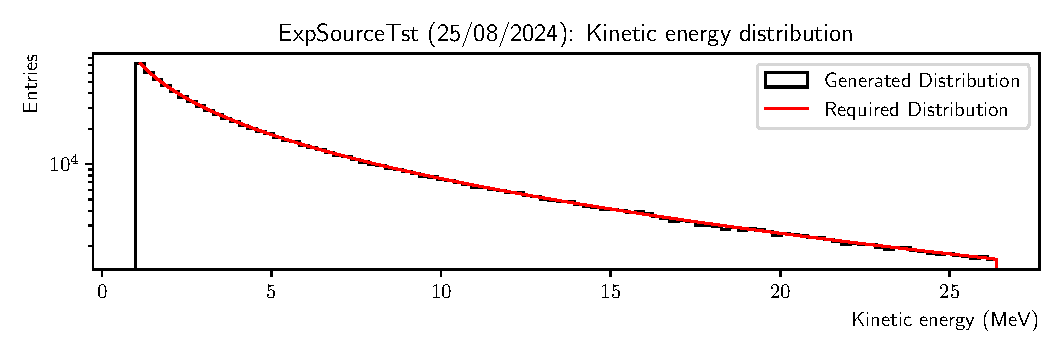
\includegraphics[width=0.92\linewidth]{SourceTst_K.pdf}
    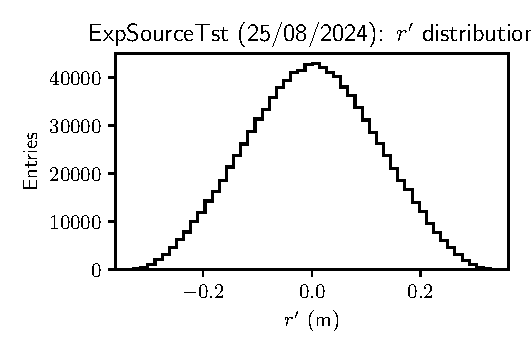
\includegraphics[width=0.46\linewidth]{SourceTst_rp.pdf}
    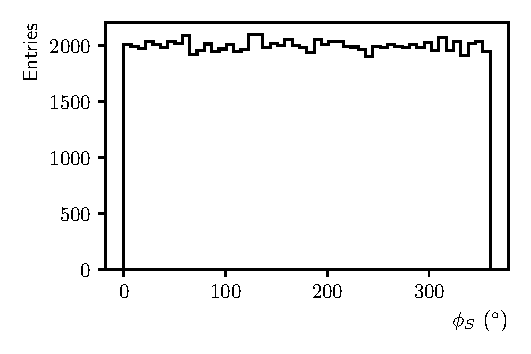
\includegraphics[width=0.46\linewidth]{SourceTst_phi.pdf}
    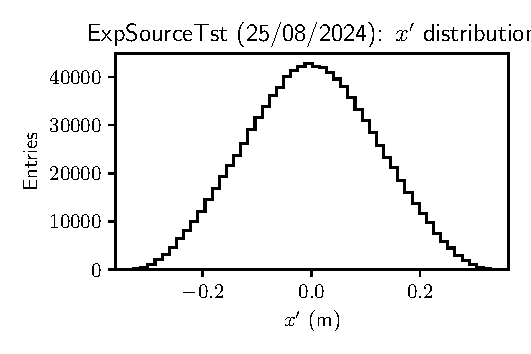
\includegraphics[width=0.46\linewidth]{SourceTst_xp.pdf}
    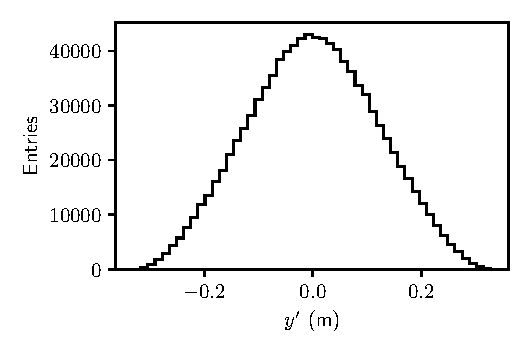
\includegraphics[width=0.46\linewidth]{SourceTst_yp.pdf}
    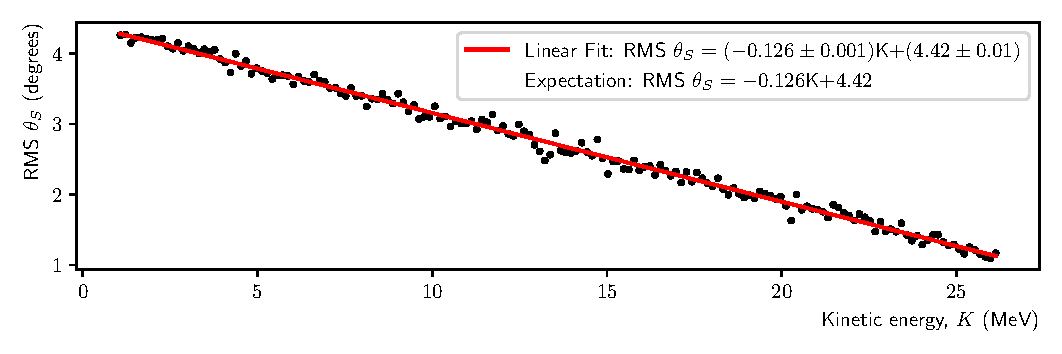
\includegraphics[width=0.92\linewidth]{RMS_Set_kE.pdf}
  \end{center}
  \caption{Kinematic distributions of particles at the point of
    production.
    \underline{Top:} The generated kinetic energy distribution is shown
    as the solid histogram. 
    The required distribution (equation~\ref{Eq:Spct:0}), normalised
    to the lowest kinetic-energy bin, is shown as the solid red line.
    \underline{Second row:} Generated $r^\prime$ and $\phi_S$
    distributions. 
    \underline{Third row:} Generated $x^\prime$ and $y^\prime$
    distributions. 
    \underline{Bottom:} RMS of the $\theta_S$ distribution versus
    kinetic energy.
    The solid circles are calculated using slices of width 0.15\,MeV.
    The red line shows the result of a straight line fit to the data.
    The expected dependence from integration of
    equation~\ref{Eq:sigVeps} is presented in the legend.
  }
  \label{Fig:LsrDrvSrc:Dists}
\end{figure}

\begin{figure}
  \begin{center}
    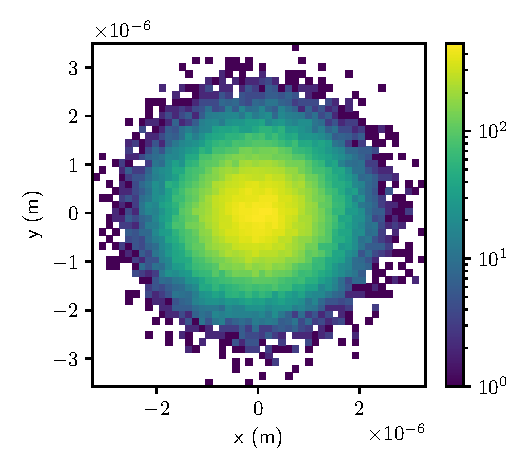
\includegraphics[width=0.46\linewidth]{SourceTst_xy.pdf}
    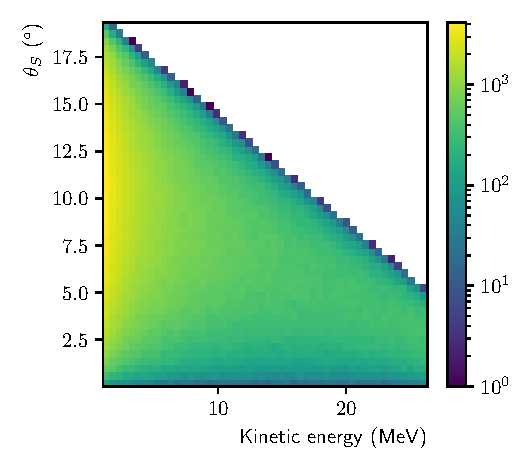
\includegraphics[width=0.46\linewidth]{SourceTst_thetaK.pdf}
    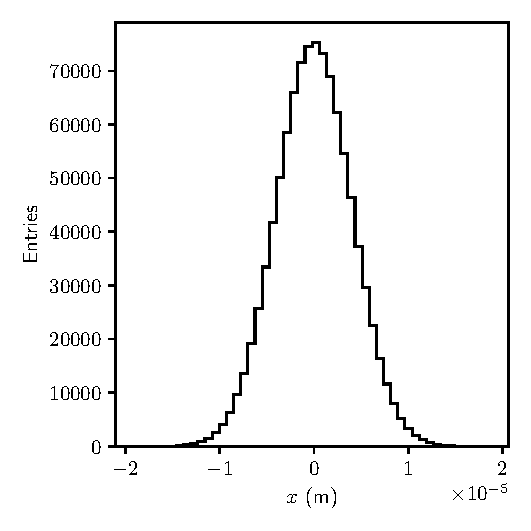
\includegraphics[width=0.46\linewidth]{SourceTst_x.pdf}
    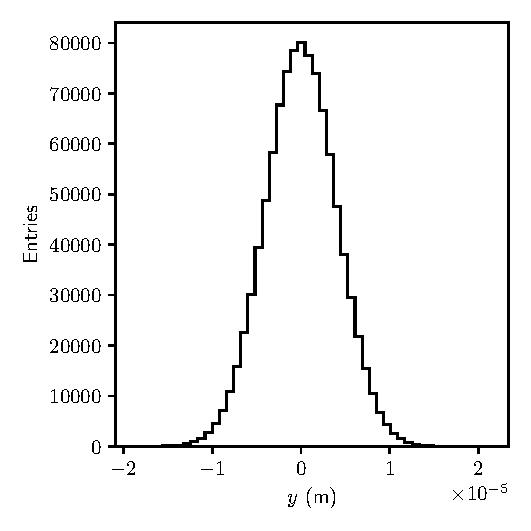
\includegraphics[width=0.46\linewidth]{SourceTst_y.pdf}
    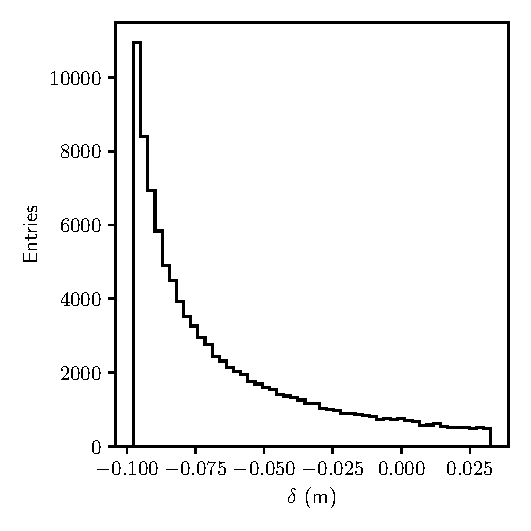
\includegraphics[width=0.46\linewidth]{SourceTst_d.pdf}
    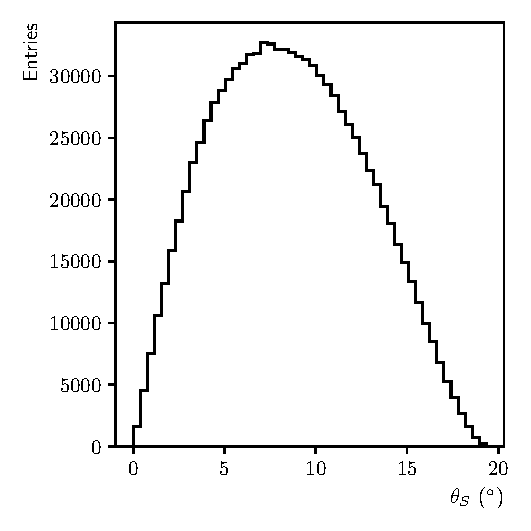
\includegraphics[width=0.46\linewidth]{SourceTst_theta.pdf}
  \end{center}
  \caption{
    \underline{Top left:} Generated $(x, y)$ distribution of the
    particle-production point.
    \underline{Top right:} The distribution of $\theta_S$ versus
    kinetic energy.
    \underline{Centre left, right:} Generated distributions of
    $x^\prime$ and $y^\prime$.
    \underline{Bottom left:} Generated distribution of $\delta$.
    \underline{Bottom right:} Generated distribution of $\theta_S$.
  }
  \label{Fig:LsrDrvSrc:Dists}
\end{figure}

\subsection{Simulated distributions}

Distributions $10^6$ protons produced by the TNSA mechanism using the
algorithm described above are shown in
figure~\ref{Fig:LsrDrvSrc:Dists}.
The parameters used in the algorithm are presented in
table~\ref{Tab:Src:Param}.
The generated distribution of kinetic energy is in good agreement with
the distribution implied by equation~\ref{Eq:Spct:0}.
The width of the generated polar-angle distribution is observed to
fall with kinetic energy and the kinetic-energy dependence of the RMS
calculated from the generated particles is in good agreement with that
expected from equation~\ref{Eq:sigVeps}.
As a result, the distribution of $\theta_S$ is approximately Gaussian
with a width dominated by the contribution of protons with kinetic
energy close to $K_{\rm min}$.
The generated $\phi_S$ distribution is flat in the range
$0^\circ < \phi_S < 360^\circ$ and the $(x, y)$ distribution is
Gaussian in both the $x$ and $y$ projections.
\begin{table}
  \caption{
    Parameters used to generate the proton phase space using
    the model described in the text.
    The parameters above the line were used to specify the model.
    The paramters below the line were calculated using the procedures
    described in the text and are representative of the J-KAREN-P
    laser that underpins the analysis in~\cite{DOVER2020100847}.
  }
  \label{Tab:Src:Param}
  \begin{center}
    \begin{tabular}{|l|c|l|}
      \hline
        \textbf{Parameter} & \textbf{Value} & \textbf{Unit} \\ 
        \hline
        Laser wavelength&0.8&$\mu$m \\ 
        Laser power&$2.5\times10^{14}$&W \\ 
        Strehl ratio&0.6& \\ 
        $r_0$&1.5e-06&$\mu$m \\
        Laser pulse duration&40e-15&s \\ 
        $K_{\rm min}$&1.0&MeV \\
        Target thickness&5&$\mu$m \\
        Electron divergence angle&25.0&degrees \\
        Intercept of RMS $\theta_S$ at $K=0$\,MeV & 20 & degrees \\
        Change of RMS $\theta_S$ between $K=0$\,MeV and $K_{\rm max}$
                            & 17 & degrees \\
      \hline
        $T_e$&12.21&MeV \\
        $K_{\rm max}$&26.34&MeV \\
      \hline
    \end{tabular}
  \end{center}
\end{table}
